% !TEX TS-program = pdflatex
% !TEX encoding = UTF-8 Unicode

% This is a simple template for a LaTeX document using the "article" class.
% See "book", "report", "letter" for other types of document.

\documentclass[11pt]{article} % use larger type; default would be 10pt

\usepackage[utf8]{inputenc} % set input encoding (not needed with XeLaTeX)

%%% Examples of Article customizations
% These packages are optional, depending whether you want the features they provide.
% See the LaTeX Companion or other references for full information.

%%% PAGE DIMENSIONS
\usepackage{geometry} % to change the page dimensions
\geometry{a4paper} % or letterpaper (US) or a5paper or....
% \geometry{margin=2in} % for example, change the margins to 2 inches all round
% \geometry{landscape} % set up the page for landscape
%   read geometry.pdf for detailed page layout information

\usepackage{graphicx} % support the \includegraphics command and options

% \usepackage[parfill]{parskip} % Activate to begin paragraphs with an empty line rather than an indent

%%% PACKAGES
\usepackage{booktabs} % for much better looking tables
\usepackage{array} % for better arrays (eg matrices) in maths
\usepackage{paralist} % very flexible & customisable lists (eg. enumerate/itemize, etc.)
\usepackage{verbatim} % adds environment for commenting out blocks of text & for better verbatim
\usepackage{subfig} % make it possible to include more than one captioned figure/table in a single float
% These packages are all incorporated in the memoir class to one degree or another...

%%% HEADERS & FOOTERS
\usepackage{fancyhdr} % This should be set AFTER setting up the page geometry
\pagestyle{fancy} % options: empty , plain , fancy
\renewcommand{\headrulewidth}{0pt} % customise the layout...
\lhead{}\chead{}\rhead{}
\lfoot{}\cfoot{\thepage}\rfoot{}

%%% SECTION TITLE APPEARANCE
\usepackage{sectsty}
\allsectionsfont{\sffamily\mdseries\upshape} % (See the fntguide.pdf for font help)
% (This matches ConTeXt defaults)

%%% ToC (table of contents) APPEARANCE
\usepackage[nottoc,notlof,notlot]{tocbibind} % Put the bibliography in the ToC
\usepackage[titles,subfigure]{tocloft} % Alter the style of the Table of Contents
\renewcommand{\cftsecfont}{\rmfamily\mdseries\upshape}
\renewcommand{\cftsecpagefont}{\rmfamily\mdseries\upshape} % No bold!

\usepackage{hyperref}
\usepackage{amsmath}


%%% END Article customizations

%%% The "real" document content comes below...

\title{Generating Instructions in Virtual Environments\\ as a Planning Problem}
\author{Yehuda Katz, Phil Nguyen, Peratham Wiriyathammabhum}
%\date{} % Activate to display a given date or no date (if empty),
         % otherwise the current date is printed 

\begin{document}
\maketitle

\begin{abstract}
In this project, we aim to create a Natural Language Generation system
that gives instructions in a virtual world at different levels of abstractions.
We incorporate a hierarchical planner into the Potsdam Natural Language Generation system,
which originally uses forward search for planning.
\end{abstract}

\section{Introduction}
The Challenge on Generating Instruction in Virtual Environment (GIVE) \cite{koller2010first}
% Phil: TODO I don't understand the phrase ``evaluation shared task''
is an evaluation shared task for real-time natural language generation (NLG) systems.
The system's objective is guiding a human instruction follower (IF) to complete a treasure-hunting task
in a 3D virtual world.
We are interested in GIVE-2.5 \cite{striegnitz2011report}, a recent version of GIVE.
GIVE-2.5 is the second sequel to GIVE and is an identical challenge
to GIVE-2 \cite{koller2010report} but was held again for a better timing.
% Phil: TODO what does the above mean?

To start the 3D game, the user downloads the 3D from the website.
The 3D client then connects to the NLG system.
There are 3 evaluation worlds with different levels of difficulty as described in figure~\ref{fig:layout}.
World 1 has a simple layout with easily identified buttons.
World 2 has many same-colored buttons, but the user can refer
to the room by the colors of the furnitures.
World 3 has a maze-like layout in one room, multiple alarm tiles
% Phil: what does ``multiple alarm tiles'' mean?
in another room,
and multiple doors with a lot of plants in the last room.

\begin{figure}[hbt!]
\centering
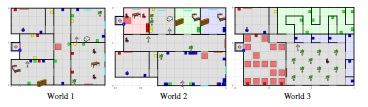
\includegraphics[width=120mm]{images/layout.jpg}
\caption{The layout of the 3 worlds in the GIVE-2.5 evaluation world \cite{striegnitz2011report}.\label{overflow}}
\label{fig:layout}
\end{figure}

The user's task is picking up a trophy from a safe after pushing a sequence of buttons.
There are obstacles such as floor tiles that can generate an alarm signal,
which unless deactivated in advance, causes the user to lose the game.
In addition, the NLG system uses many objects such as lamps and plants as landmarks.
The demo can be found at \url{https://www.youtube.com/watch?v=0RSin0HChno}.

GIVE's main difference from its sequels is in the user's movements.
In GIVE, these are discrete steps, so `taking three steps' and `turning left' are precise actions.
On the other hand, in GIVE-2 and GIVE-2.5, the user moves more freely,
so the effects of such phrases are more difficult to predict.

We are interested in the Potsdam NLG systems \cite{garoufi2011potsdam}
because they use AI planning technologies for NLG.
However, there are modifications to be tried.
For example, the Potsdam NLG systems use Forward Search (FF),
so their outputs come in one flat level of details.
We expect the use of a hierarchical planning enables outputting instructions
at multiple levels of abstraction, making the system more practical
for multiple audience.

\section{Technical Approach}

The Potsdam NLG system \cite{garoufi2011combining, garoufi2011potsdam, garoufi2014generation}
is based on the CRISP system \cite{crisp07},
which is an approach to generate natural language as a planning problem.
The CRISP system can generate individual noun phrases.
A follow up work \cite{scrisp-10} enables the system to generate an entire discourse.

The authors' contribution is transforming the tree-adjoining grammar (TAG)
into the Planning Domain Definition Language (PDDL).
Next, they use fast forward search \cite{hoffmann:nebel:jair-01} to generate
a dialog plan, which outputs a sequence of lexicons according to preconditions
from both linguistics and non-linguistics context.
An off-the-shelf planner organizes the lexicons into correct
and distinguishing descriptions of the objects in context.
Figure~\ref{fig:exampleTAG} depicts an example of the CRISP system,
which converts the TAG grammar to the planning problem for a phrase `the red button'.

\begin{figure}[hbt!]
\centering
\subfloat[TAG grammar for `the red button' which refers to the button `b1'.]{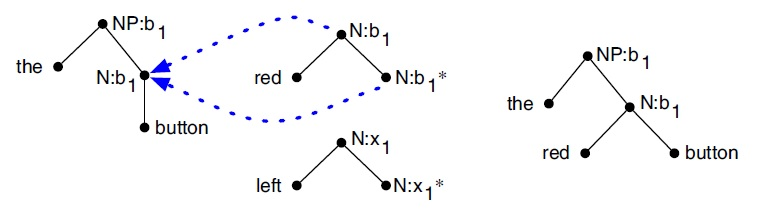
\includegraphics[width = 88mm]{images/tag.jpg}}
\qquad
\subfloat[The planning problem as preconditions and effects of lexicons `red', `left' and `the-button'.]{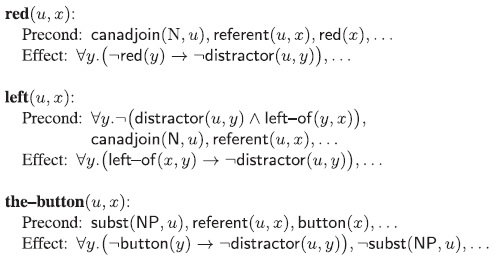
\includegraphics[width = 88mm]{images/cond.jpg}}
\caption{An example of TAG, preconditions and postconditions for some lexicons \cite{garoufi2014generation}. \label{overflow}}
\label{fig:exampleTAG}
\end{figure}

Evaluation is performed both manually and automatically \cite{garoufi2014generation}.
Manual evaluation measures how well the user follows the instructions
% TODO
as IF which may be in term of success rate or how fast the users can solve the task.
Our project is small, so we lean towards automatic evaluation.
% TODO don't use cite as noun
\cite{garoufi2014generation} proposes a maximum entropy model for automatic evaluation,
which models the success rate $P(succ(r) = 1|r,s)$ from the attribute
types in the sentence $a_j(r)$ according to a referential scene $c_i(s)$. 

\begin{equation} \label{auto_eqn}
P(succ(r) = 1| r, s) =\frac{1}{e^{\sum_j (v_j(s)*a_j(r) + w_0)} + 1} ,
\end{equation}

where $v_j(s) = \sum_i w_{ij} * c_i(s)$.
The weights $w_{ij}$ are estimated from the corpus.
Reusing the trained model may be a good choice.

\section{Project Management}

Task to Accomplish:
\begin{itemize}
  \item Set up the client, NLG server, and the matchmaker.
  \item Understand the NLG system implementation.
  \item Make a hierarchical planner version of their NLG system.
  \item Compare the results.
\end{itemize}


\noindent
Timeline:

\begin{description}
  \item[March] \hfill \\
  Set up the client, NLG server and the matchmaker.
  \item[March] \hfill \\
  Understand their NLG system implementation.
  \item[April] \hfill \\
  Make a hierarchical planner version of their NLG system.
  \item[April] \hfill \\
  Compare the results.
  \item[May] \hfill \\
  Write summary paper.
\end{description}

\section{Conclusion}
We will try to rebuild the GIVE-2.5 challenge evaluation system.
We also pick up the Potsdam NLG system which use AI planning techniques.
We try to compare hierarchical planner with their conventional fast forward search (FF). 


\bibliographystyle{plain}
\bibliography{project_proposal}

\end{document}
